\chapter{Analyse}\label{sec:analyse}

\section{Systemsekvensdiagram}
SSD-diagrammet adresserer, hvordan brugeren og systemet kommunikerer frem og tilbage. Dette SSD-diagram er lavet ud fra Fully Dressed Use Case, automatisk lagerstyring.

\begin{figure}
    \centering
    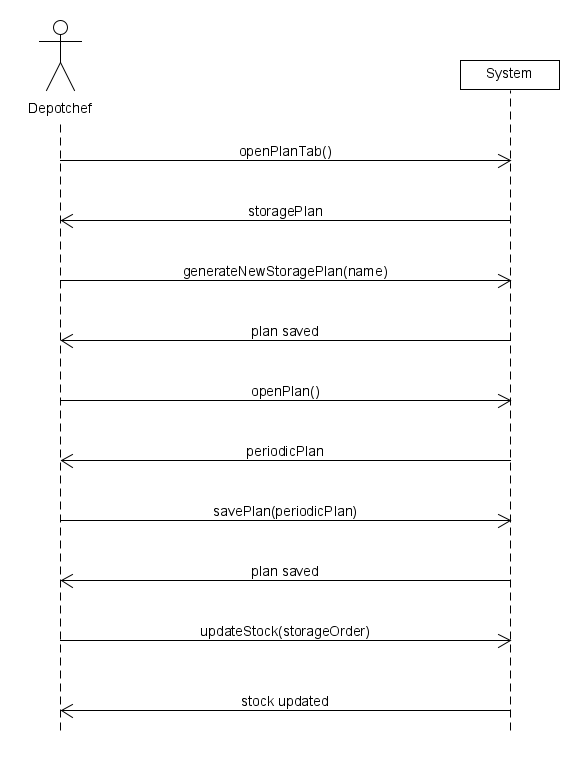
\includegraphics[width=50mm]{figures/analyse/SSD.png}
    \caption{Systemsekvensdiagram}
    \label{fig:ssd}
\end{figure}

Her ses det, at depotchef Niels Thomas er den eneste, som benytter systemet. Som det første åbner Niels Thomas den nuværede plan for lageret, hvorefter vil systemet give den nuværende lager plan. 

Når den er åbnet kan Niels Thomas generere en ny lager plan \verb|generateNewStoragePlan(name)|, samt navngive planen. Denne funktion generer en plan, baseret på salgsdata, produkters popularitet og kommende udsalg. Når planen er genereret, vil den blive ved med at oprette storageOrders, baseret på den oprettede plan. 
Såfremt planen har brug for ændring, skal der genereres en ny plan. Det er muligt at åbne den og foretage ændringer i planen. Et eksempel kunne være, at man ville have 20 isbåde istedet for 10. Herefter gemmes planen og storageOrders oprettes automatisk på ubestemt tid. 

 
\section{Operationskontrakt}
\todo{write stuff about operationskontrakt}
Ud fra SSD diagrammet og Fully Dressed Use Casen kan der udvikles en operationskontrakt. Operationskontrakten beskriver i flere detaljer hvad der sker af ændringer i programmet under hvert trin i use casen. Noget som ikke fremkommer tydeligt under disse trin er, at så snart en PeriodicPlan er oprettet, vil denne oprette en StorageOrder som er en varebestilling.
%remember to talk about the autogeneration continuation process thing algorithm stuff :) 

\begin{center}
    \begin{longtable}{ |p{360pt}| }
        \hline
        \textbf{Operationskontrakt}
        \\
        \noindent\fbox{%
            \parbox{4.88in}{%
                \textbf{Operation:} openPlanTab() \\ Åbner planfanen i programmet
                
            }%
        }

        \noindent\fbox{%
            \parbox{4.88in}{%
                \textbf{Operation:} generateNewStoragePlan(name) \\ 
                Use Case: Bestil Varer \\

                Præ-betingelser: en instans af productMap eksisterer \\

                Post-betingelser: \\
                - sp.name blev sat til name \\
                - En instans af PeriodicPlan blev oprettet \\
                - pp.period blev sat til period \\
                - en instans af sOrder blev oprettet \\
                - pp blev associeret med product og sOrder \\
                - p blev associeret med supplier og productLine \\
                - sOrder blev associeret med supplier og productLine 
            }%
        }

        \noindent\fbox{%
            \parbox{4.88in}{%
                \textbf{Operation:} openPlan() \\
                Den generede plan åbnes i planfanen i programmet
            }%
        }
        
        \noindent\fbox{%
            \parbox{4.88in}{%
                \textbf{Operation:} savePlan(periodicPlan) \\
                Use Case: CRUD StoragePlan \\
                Præ-betingelser: En instans af StoragePlan eksisterer \\
                Post-betingelser: \\
                - De nye periodicPlan instanser gemmes i periodicPlans
            }%
        }

        \noindent\fbox{%
            \parbox{4.88in}{%
                \textbf{Operation:} updateStock(storageOrder)
                Use Case: Modtag Varer \\
                Præ-betingelser: Produkterne bestilt fra en storageOrder er ankommet til depotet. \\
                Post-betingelser: \\
                - sOrder.sentDate er blevet sat til sentDate \\
                - sOrder.trackingId er blevet sat til trackingId \\
                - productLine.amount er blevet opdateret
            }%
        }
        
    \end{longtable}
\end{center}





